%
% ---------- chapter 4 ----------
%

\section{Design of Algorithm}
%
This paper aims to solve above-mentioned project management problem by using
evolutionary algorithm. There are two important steps in using the evolutionary
algorithm. One is to choose the representation of the problem's solution, the
other is to define a appropriate fitness function.

%% \begin{figure}[!ht]
%%   \centering
%%   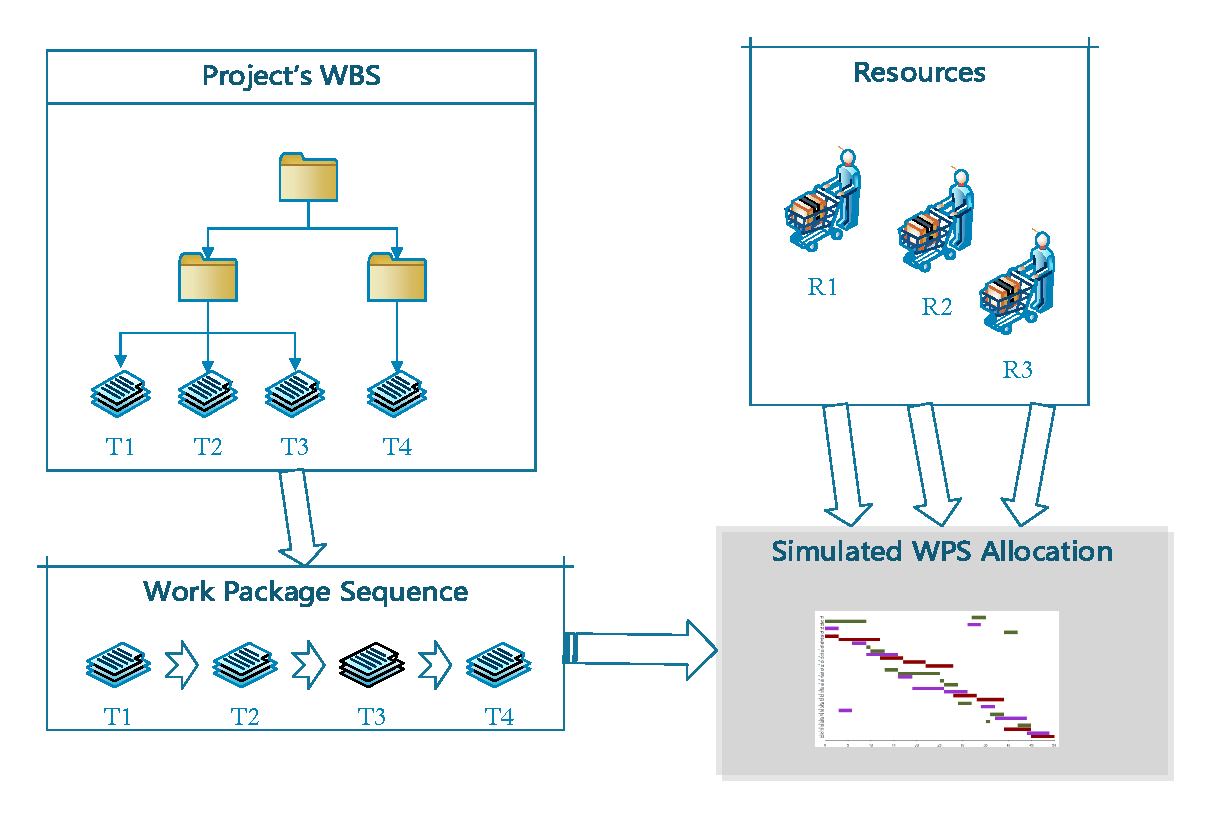
\includegraphics[width=0.8\textwidth]{figures/simu.pdf}
%%   \caption{Project Plan of Software Development}
%%   \label{fig:simu}
%% \end{figure}

%% There are two important steps in using the evolutionary algorithm. One is to
%% choose the representation of the problem's solution, the other is to define a
%% appropriate fitness function. In the process of project management, the work
%% packages in the project are allocated by simulation. See figure \ref{fig:simu},
%% Firstly, the whole project is decomposed into several work packages by
%% \emph{work breakdown structure}, and those work packages are arranged into a
%% corresponding \emph{work package sequence}. Secondly, according to the
%% dependencies of the work packages and the restriction of resource, each kinds of
%% resources is allocated to the corresponding work package by
%% \emph{first-come-first-served} algorithm. Finally, the project's overall
%% duration is calculate by simulation.


\subsection{The Representation of Solution}
%
For the above-mentioned problem, the representation of solution is defined as
follows.


This paper uses \emph{work package sequence} (hereinafter referred to as \emph{WPS}) to
represent a solution of project management problem. The representation of such a
solution is actually a priority arrangement sequence of the work packages in
the whole project, and the number of solutions for a project containing the $N$
work packages is $N!$, which is large enough to do random search.

%This is a figure 7
\begin{equation}
  T_1 \rightarrow T_5 \rightarrow T_6 \rightarrow T_4 \rightarrow T_8
  \rightarrow T_3 \rightarrow T_9 \rightarrow T_2 \rightarrow T_7
  \label{repr}
\end{equation}

For example, equation (\ref{repr}) is solution, the solution represents the work
package sequence in the priority of $T_1$, $T_5$, $T_6$, $T_4$, $T_8$, $T_3$,
$T_9$, $T_2$, $T_7$, while arranging the work packages. This representation is
beneficial and intuitive to programming.


\subsection{Fitness Evaluation}
%
The above-mentioned representation of solution make each individual coded as
\emph{WPS}. The fitness value of \emph{WPS} is the project's overall duration,
which is calculated by simulating the assignment of work packages in the set of
package sequence, see equation (\ref{wps}).

For each \emph{WPS}, the algorithm to calculate corresponding project overall
duration is as follows. Firstly, according to first-come-first-served (FCFS)
rule, the front work packages in a \emph{WPS} have high priority to get
resources, the back work packages has low priority. Secondly, the $TR$ function
defines which work package can get which resources, if two work packages that
require the same resources, the higher priority one will use the resources
firstly, the lower priority one will use the resources after the higher one
releases the resources. Finally, the project's overall duration is the last end
time after all work packages are allocated the resources (see algorithm
\ref{alg}).


\begin{algorithm}
  \caption{Fitness Evaluation Algorithm}
  \label{alg}
  \begin{algorithmic}
    \REQUIRE $WPS, R, TE, TR$
    \ENSURE $duration$
    \FOR {$i$ \textbf{from} $1$ \textbf{to} $WPS.length$}
      \STATE $t \gets WPS[i]$
      \STATE $ effort \gets TE(i)$
      \FOR {$r$ \textbf{in} $R$}
        \STATE $r.occupy \gets 0$
      \ENDFOR 
      \FOR {$r$ \textbf{in} $R$}
        \IF{$TR(t,r) = true$}
          \STATE $t.start \gets r.occupy$
          \STATE $t.end \gets r.occupy + effort$
          \STATE $r.occupy \gets t.end$
          \STATE \textbf{break}
        \ENDIF
      \ENDFOR
    \ENDFOR
    \STATE $duration \gets 0$  
    \FOR {$t$ \textbf{in} $WPS$}
      \IF{$t.end > duration$}
        \STATE $duration \gets t.end$
      \ENDIF
    \ENDFOR
  \end{algorithmic}
\end{algorithm}

\subsection{Genetic Operators}
%

There are two main types of operators in evolutionary algorithms:
\emph{crossover} and \emph{mutation}.

\subsubsection{Crossover}
In evolutionary algorithms, crossover is a genetic operator used to vary the
programming of a chromosome or chromosomes from one generation to the next.  In
this paper, we use a two-point crossover, that is, two points are selected
randomly on the parent organism strings. Everything between the two points is
swapped between the parent organisms, rendering two child organisms then
exchange corresponding part of chromosomes to get offspring individual.


\subsubsection{Mutation}
In evolutionary algorithms, Mutation is a genetic operator used to maintain
genetic diversity from one generation of a population of genetic algorithm
chromosomes to the next.  In this paper, we use two-point exchange mutation,
that is, two points is selected randomly on individual organisms strings, and
then exchange the two points.


\subsection{Parallel Evolutionary Algorithm}
%
Figure \ref{fig:flow} summarizes the basic process of the evolutionary
algorithm.


\begin{figure}[!ht]
  \centering
  % fisrt figure
  \begin{minipage}{0.29\textwidth}
    \centering
    \subfigure[Sequential] {
      \label{fig:flow:s}
      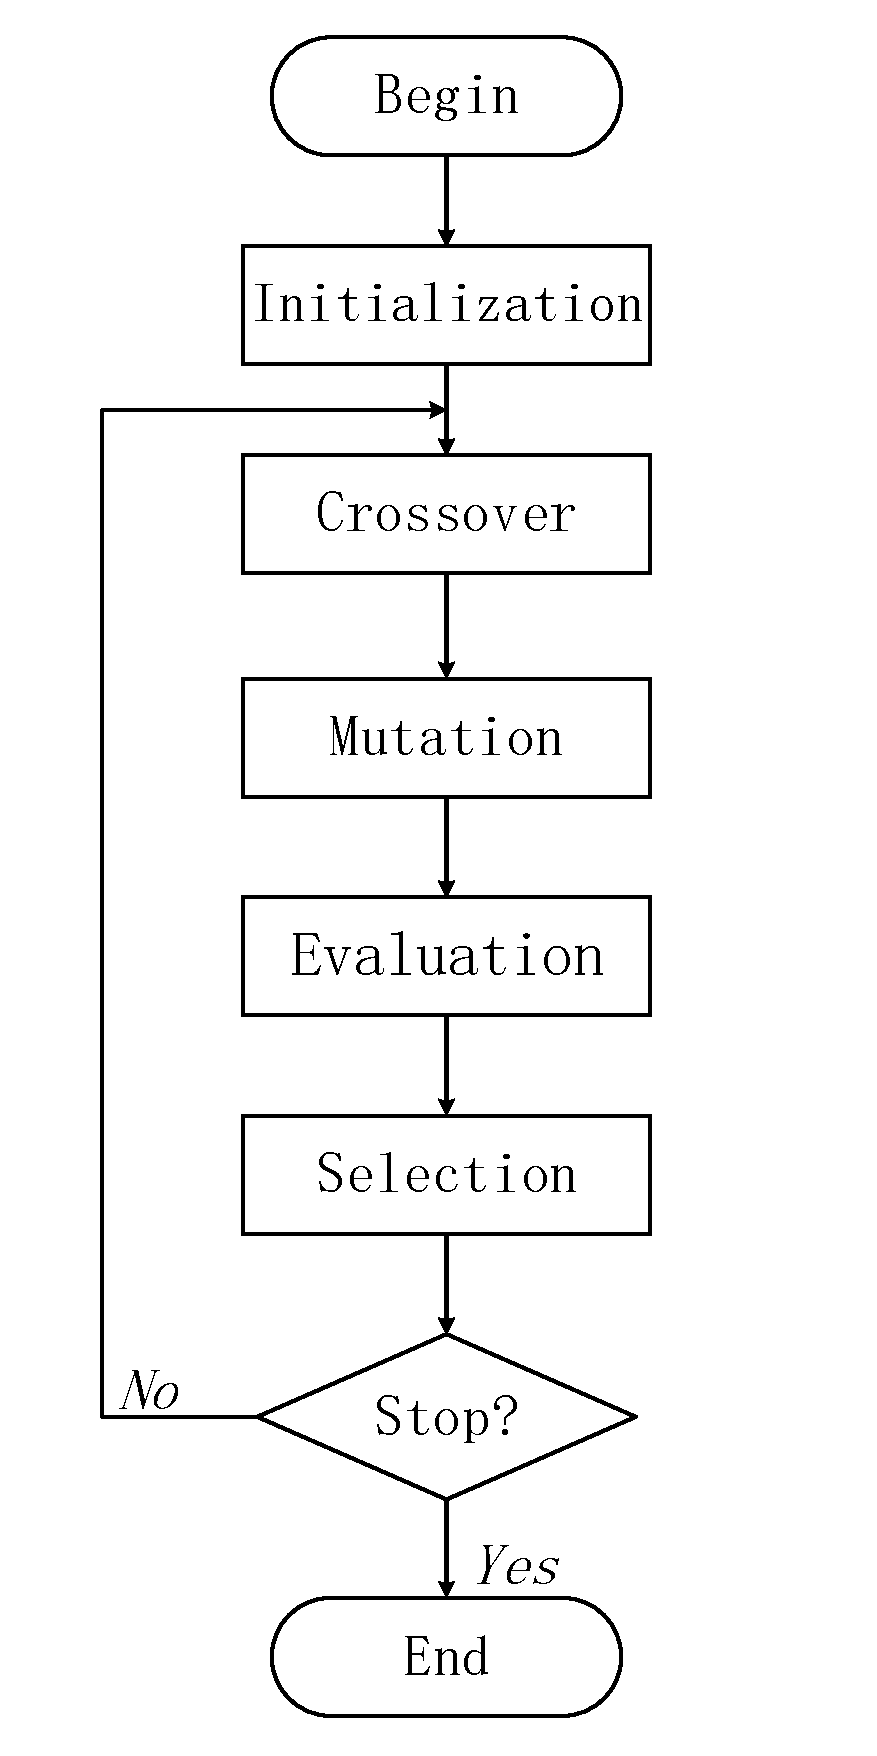
\includegraphics[width=\textwidth]{figures/ea_flow.pdf}
    }
  \end{minipage}
  % second figure
  \begin{minipage}{0.58\textwidth}
    \centering
    \subfigure[Parallel] {
      \label{fig:flow:p}
      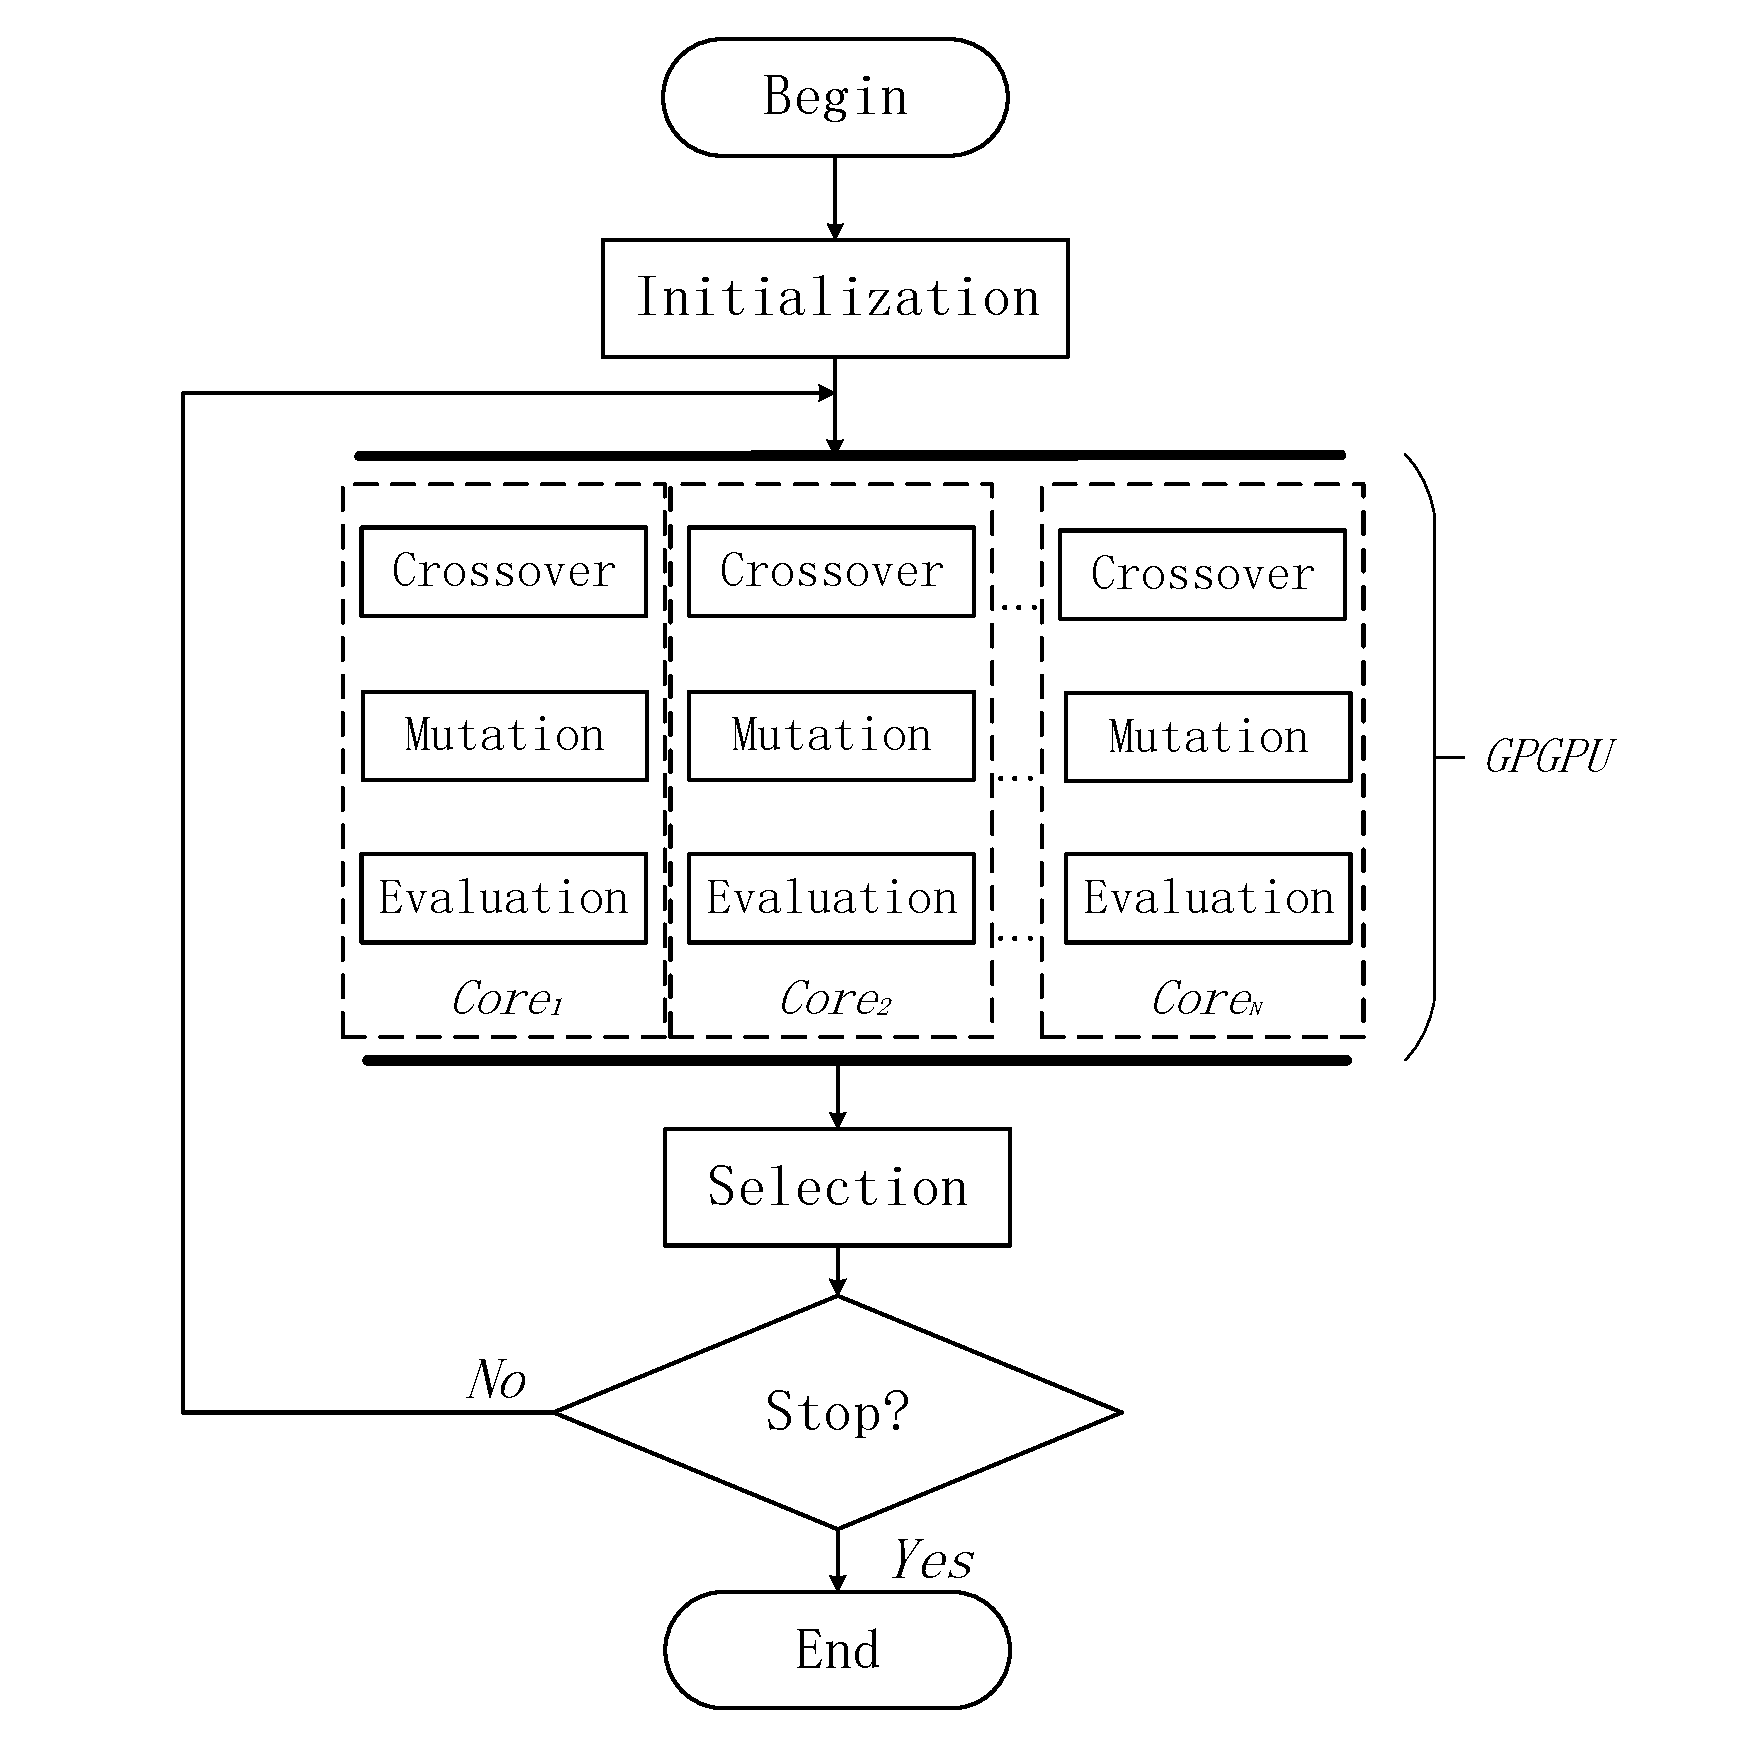
\includegraphics[width=\textwidth]{figures/ea2_flow.pdf}
    }
  \end{minipage}
  \caption{Sequential and Parallel Evolutionary Algorithm}
  \label{fig:flow}
\end{figure}


Figure \ref{fig:flow:s} is common sequenctial evolutionary algorithm, the
algorithm has several steps, such as initialization, crossover, mutation, and
selection. Candidate solutions to the optimization problem play the role of
individuals in a population, and the fitness function determines the convergence
of the solutions. Evolution of the population then takes place after the
repeated application of the above operators.


Figure \ref{fig:flow:p} illustrates a parallel evolutionary algorithm. The
parallel one follows most steps in sequenctial one, but put the top
time-consuming work on GPU. The steps of crossover, mutation and evolution runs
in different cores in GPU so that the speed of calculation can be impoved a lot.



